\chapter{Antecedentes}
En este capítulo se presenta el contexto de las pequeñas empresas del sector de la construcción y las instalaciones de climatización. Se realizará una investigación que partira desde lo más general de la obra pública y la estructura de las PYMES del sector, hasta llegar al análisis de los procesos de gestión internos que presentan mayores ineficiencias. Asimismo, se examinará el estado actual de la tecnología en el sector, identificando las limitaciones de las herramientas tradicionales y evaluando las soluciones actuales.
\section{Ámbito de la obra pública en el sector aeroportuario}
La empresa se centra en el ámbito concreta de la obra publica aeroportuaria, el cual es un entorno altamente regulado, donde la carga administrativa suele superar la capacidad técnica de las pequeñas empresas. En esta sección se analizarán los mecanismos de licitación pública y los requisitos específicos de seguridad que condicionan la operativa diaria en infraestructuras críticas, basándose en el marco normativo vigente \cite{SEDIA2026}.
Las empresas que operan en el sector público deben participar en procesos de \textbf{licitación} convocados por diversos organismos e instituciones (ayuntamientos, ministerios, entes públicos, etc.). Este proceso sigue una estructura específica que marca el inicio de cualquier proyecto.En la figura \ref{fig:proceso_licitacion} podemos observar un diagrama de flujo, donde podemos ver las multiples fases del proceso que van desde el analisis de la licitación hasta la adjudicación de esta.
\newpage
\begin{figure}[h]
    \centering
    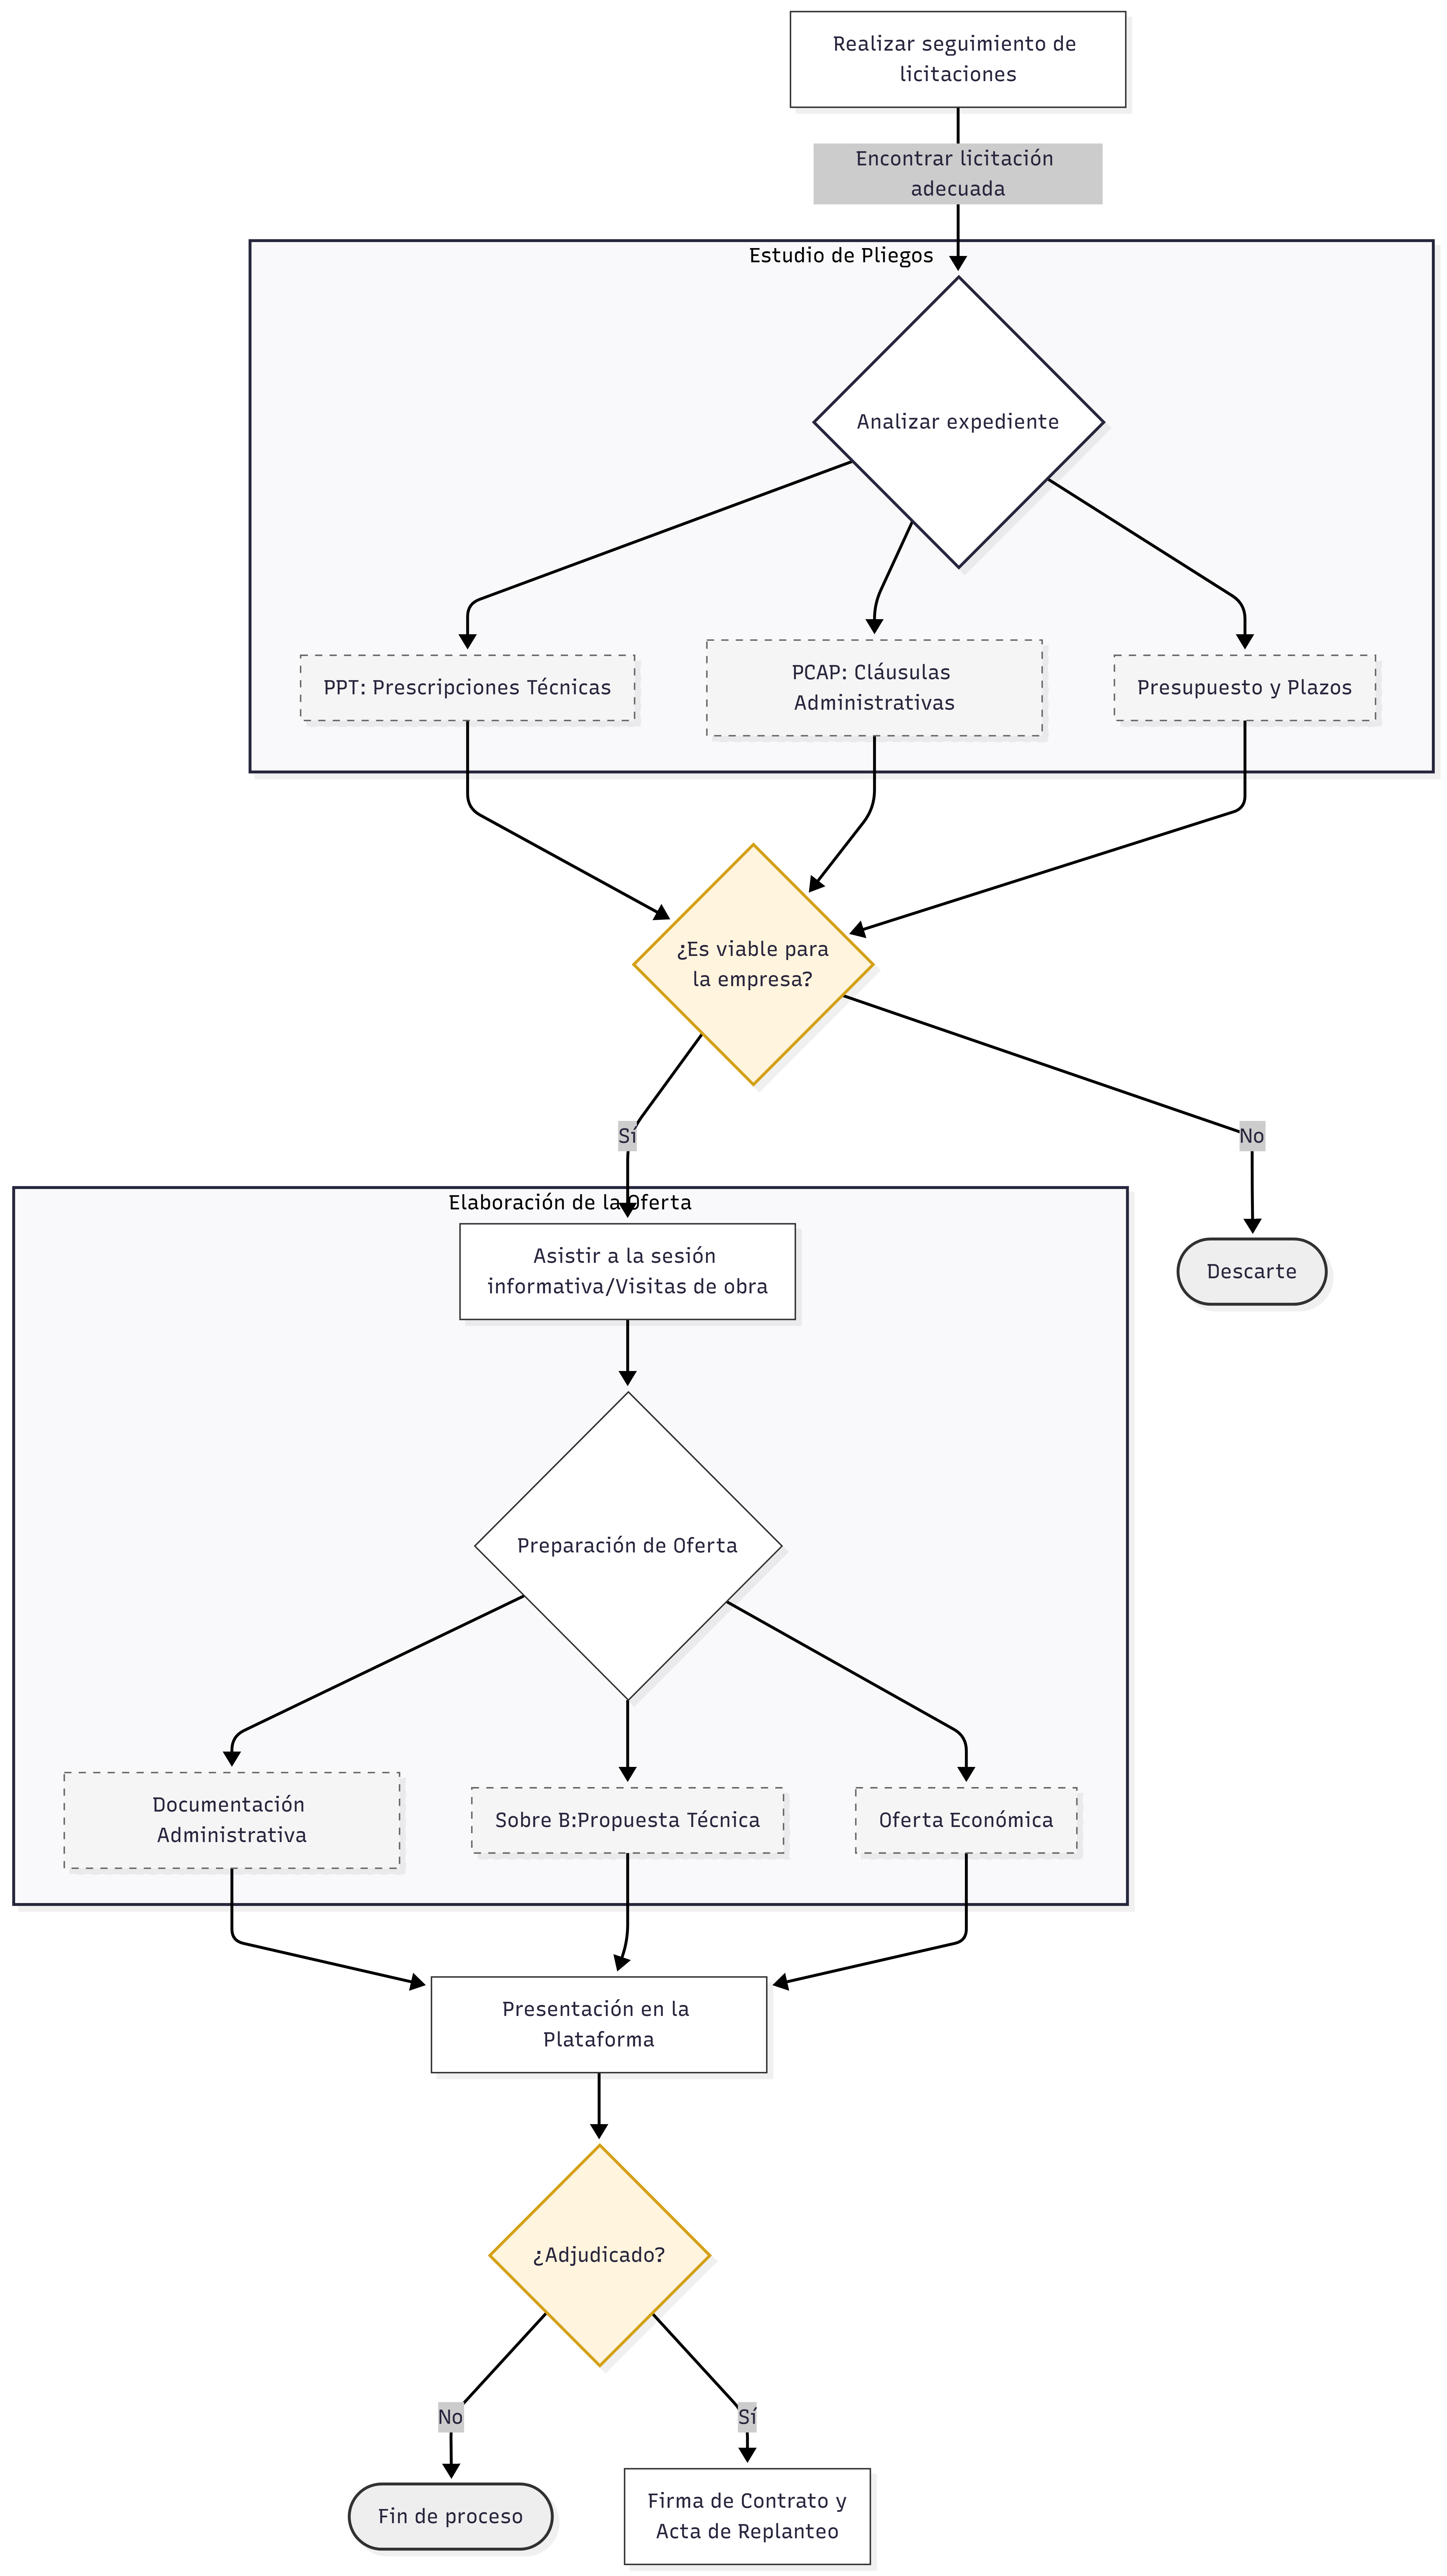
\includegraphics[width=0.65\textwidth]{figs/Procesos de licitación.png} 
    \caption{Diagrama de flujo del proceso de licitación}
    \label{fig:proceso_licitacion}
\end{figure}
\subsection{Marco administrativo y licitación pública}

\begin{figure}[ht]
    \centering
    \includegraphics[width=0.8\textwidth]{figs/construccion_aeropuerto.jpg}
    \caption{Obras de expansión en infraestructura aeroportuaria. Fuente: Olaf Tausch vía Wikimedia Commons (Licencia CC BY-SA 3.0).}
    \label{fig:construccion_aeropuerto}
\end{figure}
El canal principal en el cual poder encontar licitaciones públicas es la \textit{Plataforma de Contratación del Sector Público}, en la cual, diversas administraciones públicas ofertán un proyecto. Cuando se pública una licitación, es procesada como un \textbf{expediente} administrativo.
Cada expediente representa un proyecto licitado por la administración y se identifica mediante un número de identificación único. Este registro contiene información importante, tal como la fecha límite de presentación, el importe base de licitación, la descripción técnica y, fundamentalmente, el \textbf{pliego}. Este documento detalla las actuaciones a realizar y los requisitos técnicos y legales que la empresa debe cumplir para ser considerada apta.
Tras haber comentado los activos principales,se explicará la fase de busqueda de expedientes desde el punto de vista de las empresas. Las empresas analizan detalladamente el pliego para evaluar la viabilidad del proyecto, comprobando las actuaciones requeridas, la rentabilidad económica y los plazos de presentación. Si estas condiciones se ajustan a la capacidad e intereses de la entidad jurídica, se procede con la preparación de la oferta.
Para preparar la oferta, se deberá de recopilar cierta información, las empresas suelen obtenerla a través de la \textbf{presentación} del expediente, junto con visitas a la obra. Después de haber preparado la oferta, la cual contendrá una extensa documentación administrativa, junto con la oferta económica detallada para cada actuación descrita en el pliego, la administración publicadora evaluará todas las ofertas, y seleccionarán la mejor. Finalmente, en ese momento, podemos decir que la licitación ha sido\textbf{adjudicada}.
\subsection{Gestiones administrativas en entornos aeroportuarios}
Una vez adjudicada la obra, las labores en el recinto aeroportuario presentan diversas complicaciones, que se deben a las nomativas europeas \cite{UE_139_2014} las cuales fueron definidas por la Agencia Estatal de Seguridad Aérea (AESA) \cite{AESA_Web}. AESA actúa como el organismo regulador de la seguridad aérea en España, mientras que AENA ejerce como gestor, siendo los responsables del cumplimiento.
Los técnicos deben realizar reformas, junto con instalaciones eléctricas entre las que se incluyen las instalaciones de climatización en zonas de tránsito de pasajeros o \bft{áreas restringidas} (denominadas lado aire y lado tierra). Esto implica una serie de precauciones críticas que deben ser tratadas:
\begin{itemize}
\item{Formación Obligatoria:} Los trabajadores deben superar programas de formación específica. El curso AVSEC les capacita en la protección contra actos de interferencia ilícita \cite{AENA_AVSEC}, mientras que el AVSAF se centra en la seguridad operacional en pista \cite{AENA_AVSAF}. Sin estas certificaciones vigentes, el trabajador tiene denegado el acceso autónomo, dependiendo de acompañamiento autorizado, lo que penaliza la productividad.
\item{Logística de Accesos:} El transporte de materiales debe coordinarse con los horarios de baja operativa del aeropuerto, requiriendo escoltas o pases de seguridad temporales cuya gestión esta regida por reglas inflexibles, lo que provoca un retraso considerable.
\item{Gestión de Residuos:} El desescombro y la limpieza deben ser inmediatos y bajo normativas ambientales estrictas para no afectar a la calidad del aire o la visibilidad en terminales.
\end{itemize}
\begin{figure}[ht]
    \centering
    \includegraphics[width=0.8\textwidth]{figs/Tecnicos.jpg} 
    \caption{Operarios coordinando tareas de mantenimiento e infraestructura. Fuente: \textit{“Discussing the work”} por Oregon Department of Transportation, utilizada bajo licencia CC BY 2.0 (\url{https://creativecommons.org/licenses/by/2.0/}).}
    \label{fig:discusion_obra}
\end{figure}
\newpage
\section{Entorno digital del sector}
Una vez expuesto el marco administrativo y operativo al que se exponen las pequeñas y medianas empresas en la obra pública aeroportuaria, es de vital importancia analizar el entorno software con el que las empresas operan. En este apartado se evaluará el estado actual de digitalización del sector, identificando las carencias de las soluciones de las organizaciones y analizando las herramientas y aplicaciones que predominan actualmente en el mercado.
\subsection{Deuda técnica del sector}
A pesar de que el sector público ha avanzado hacia la administración electrónica, la digitalización en las pymes de la construcción e instalaciones presenta una evolución muy irregular \cite{ONTSI_Pymes, DESI2026}. Esta disparidad genera lo que en Ingeniería del Software se conoce como \textbf{deuda técnica}. Esta deuda se produce por el coste de mantener soluciones de software limitadas, parches temporales o arquitecturas deficientes en lugar de invertir en un sistema escalable y bien diseñado.
En el caso de estas empresas, la deuda técnica no suele provenir de código mal escrito, sino por la falta de un software especializado. Al contar con un capital limitado, siempre surge el miedo de invertir en algo nuevo que no se sabe cual va a ser su rentabilidad.
\begin{table}[h]
\centering
\renewcommand{\arraystretch}{1.2}
\begin{tabular}{|l|c|c|c|}
\hline
\rowcolor{gray!20} \bft{Sector de Actividad (2022)} & \bft{Total (\%)} & \bft{Total > 10 (\%)} & \bft{Total micro (\%)} \\ \hline
Construcción & 59,9 & 75,4 & 58,7 \\ \hline
Act. Inmobiliarias y Administrativas & 67,1 & 81,1 & 66,4 \\ \hline
\end{tabular}
\caption{Valor de la dimensión equipamientos e infraestructuras por tamaño de empresa. Fuente: Elaboración propia a partir de datos del ONTSI (2023)}
\label{tab:datos_ontsi_construccion}
\end{table}
\subsection{Soluciones software del sector}
A la hora de hablar de las soluciones software del sector, no existe una única herramienta integral que cubra todas las necesidades de una empresa. Por lo tanto, se debe abordar el ecosistema desde una perspectiva fragmentada, categorizando las aplicaciones según el area en el que se use. En la actualidad, las pymes se estructuran en los siguientes bloques software que suelen estar incomunicados entre ellos.
\subsubsection{Plataformas de licitacion}
Las empresas están obligadas a utilizar portales externos como los de AENA o los de la Plataforma de Contratación del Estado. Estas plataformas han agilizado la administración de expedientes, tanto desde el punto de vista de la entidad publicadora, como de la entidad licitadora. Sin embargo, estas webs obligana realizar procesos manuales y redundantes hacía los sistemas internos de la empresa.
%CAPTURA DE AENA O DE LA PLATAFORMA DE CONTRATACIÓN DEL ESTADO
\subsubsection{Gestión económica y facturación}
Para el cumplimiento fiscal y la contabilidad, las pymes recurren a software especializado. El principal inconveniente de estas soluciones en las pymes es que, aunque resuelven la parte administrativa, suelen quedar aisladas del resto de los procesos operativos técnicos de la obra. 
%CAPTURA FACTUSOL
Es importante destacar que este entorno va a cambiar con la inminente implantación del sistema \textbf{VeriFactu}. Impulsado por la Agencia Tributaria (AEAT) como medida antifraude, VeriFactu es un nuevo reglamento que exigirá que los programas informáticos de facturación garanticen la inalterabilidad, trazabilidad y conservación de los registros. Esto significa que el software deberá ser capaz de certificar las facturas y enviarlas automáticamente a la administración en tiempo real. 
Dado que Verifactu establece la normativa, las aplicaciones de facturación deberán adaptar su arquitectura para cumplir con las reglas impuestas. Aquellas herramientas que, por limitaciones o código heredado, no sean capaces de integrar las exigencias, quedarán obsoletas y saldrán del mercado. Esta transición obligará a muchas pymes a adoptar una nueva tecnología, lo cual generará varios problemas derivados entre los que se encuentan la curva de aprendizaje y, por consiguiente, una migración masiva de datos para el nuevo programa.
%CAPTURA DE ALGUNA NORMATIVA DE VERIFACTU
\subsubsection{Herramientas de gestión y almacenamiento de datos}
Ante la falta de sistemas centralizados, existe una tendencia generalizada en el sector a utilizar hojas de cálculo (principalmente Microsoft Excel) como herramientas principales para la gestión y almacenamiento de datos. Estos documentos asumen roles para los que no fueron diseñados, actuando como bases de datos improvisadas para el control de presupuestos, certificaciones de obra, inventario de materiales e incluso gestión de combustibles. 
Desde el punto de vista de la ingeniería del software, esta práctica genera una importante deuda técnica. Las hojas de cálculo carecen de propiedades transaccionales, no imponen restricciones de integridad referencial y presentan graves limitaciones en entornos de trabajo colaborativo o concurrente. La ausencia de un modelo de datos estructurado provoca duplicidad de información y dificulta la extracción de métricas fiables sobre el estado real de los proyectos.
%CAPTURA DE EXCEL
\subsubsection{Sistemas integrados de gestión (ERP)}
Por último, al analizar las soluciones tecnológicas del mercado, es inevitable mencionar los sistemas empresariales monolíticos, concretamente los sistemas de planificación de recursos empresariales (ERP, por sus siglas en inglés). 

En teoría, la implantación de un ERP resolvería el problema de la fragmentación de datos mencionado anteriormente, al unificar la facturación, los recursos humanos y la gestión de proyectos en una única plataforma. Sin embargo, en la práctica, estas soluciones presentan barreras de entrada críticas para las pymes del sector aeroportuario. Por un lado, suponen un coste económico y un tiempo de implantación inasumibles para empresas de tamaño reducido. Por otro lado, su arquitectura suele ser demasiado rígida para adaptarse a las particularidades y flujos de trabajo tan específicos que imponen organismos como AENA.

Por un lado, destacan los \textbf{ERPs genéricos y modulares}, entre los cuales podemos destacar Odoo, siendo una de las opciones mas valroadas por la pymes al ser Open Source. Permite a la empresa instalar únicamente las aplicaciones que necesitan. Además de Odoo, tambien existe Microsfot 365 Business central. Es el estandar corporativo,siendo robusto, pero presentando ciertas limitaciones, las principales serían sus licencias de alto coste, curva de aprendizaje y tiempos de de implantación que suelen ser meses.
%CAPTURA DE LOS ERPS
Por otro lado, existen \textbf{ERPs verticales específicos para la construcción}. Estos ERPs son soluciones diseñadas para el secotr de la construcción. Cuenta con modulos para hacer multiples gestiones como presupuestos o certificaciones de obra. De entras estas, podemos destacar Sigrid y BrickControl
%CAPTURA DE LOS ERPS
A pesar de la existencia de la existencia de estas potentes herramientas en el mercado, su adopción para empresas pequeñas es baja al presentar una arquitectura rígida que complica la adaptación a flujos de trabajo específicos. %Seguir, con el porque de que no se implemente en las pymes.
